% mn2esample.tex
%
% v2.1 released 22nd May 2002 (G. Hutton)
%
% The mnsample.tex file has been amended to highlight
% the proper use of LaTeX2e code with the class file
% and using natbib cross-referencing. These changes
% do not reflect the original paper by A. V. Raveendran.
%
% Previous versions of this sample document were
% compatible with the LaTeX 2.09 style file mn.sty
% v1.2 released 5th September 1994 (M. Reed)
% v1.1 released 18th July 1994
% v1.0 released 28th January 1994

\documentclass[useAMS,usenatbib]{mn2e}

% If your system does not have the AMS fonts version 2.0 installed, then
% remove the useAMS option.
%
% useAMS allows you to obtain upright Greek characters.
% e.g. \umu, \upi etc.  See the section on "Upright Greek characters" in
% this guide for further information.
%
% If you are using AMS 2.0 fonts, bold math letters/symbols are available
% at a larger range of sizes for NFSS release 1 and 2 (using \boldmath or
% preferably \bmath).
%
% The usenatbib command allows the use of Patrick Daly's natbib.sty for
% cross-referencing.
%
% If you wish to typeset the paper in Times font (if you do not have the
% PostScript Type 1 Computer Modern fonts you will need to do this to get
% smoother fonts in a PDF file) then uncomment the next line
% \usepackage{Times}
 \usepackage{times}

%%%%% AUTHORS - PLACE YOUR OWN MACROS HERE %%%%%

\usepackage{graphicx}
\usepackage{supertabular}
\usepackage{subfig}
\usepackage{rotating}
\usepackage{lscape}
\usepackage{epsfig}
%\usepackage{natbib}
\usepackage{amssymb}
%\usepackage{myaasmacros}
\usepackage{amsmath}
\usepackage{multicol}
%\usepackage{makecell}
\usepackage{slashbox}
\usepackage{color}

\bibliographystyle{astron}

\def\squig{$\sim\!\!$}
\def\lesssim{\mathrel{\hbox{\rlap{\hbox{\lower4pt\hbox{$\sim$}}}\hbox{$<$}}}}
\def\gtrsim{\mathrel{\hbox{\rlap{\hbox{\lower4pt\hbox{$\sim$}}}\hbox{$>$}}}}
\def\subsun{\mbox{$_{\normalsize\odot}$}}
\def\arcsec{\hbox{$^{\prime\prime}$}}
\def\arcmin{$^{\prime}$}
\def\deg{\hbox{$^\circ$}}
\def\mic{ $\mu $m\,}
%\def\power{WHz$^{-1}$sr$^{-1}$}
%\def\flux{erg s$^{-1}$ cm$^{-2}$}
%\def\lum{erg s$^{-1}$}
%\def\14{\rm 1.4\,GHz}
%\def\27{\rm 2.7\,GHz}
%\def\whz1{$\,\rm W\,Hz^{-1}$}
%\def\kms1{$\,\rm km\,s^{-1}$}

\def\aas{A\&A Sup} 
\def\apj{ApJ} 
\def\apjs{ApJSup} 
\def\mnras{MNRAS} 
\def\aaps{AAPS}
\def\pasp{PASP} 
 

%%%%%%%%%%%%%%%%%%%%%%%%%%%%%%%%%%%%%%%%%%%%%%%%

\title[MADX - A simple technique for source detection in multiband imaging]{MADX}
\author[S.J. Maddox]{\parbox{\textwidth}{S.J. Maddox$^{1}$
\thanks{E-mail: steve.maddox@nottingham.ac.uk}, L. Dunne$^{1}$}}

\begin{document}

\date{}

\pagerange{\pageref{firstpage}--\pageref{lastpage}} \pubyear{2002}

\maketitle

\label{firstpage}

\begin{abstract}
We describe a simple technique for detecting sources in multiband
imaging. The method is to filter the individual bands by the
corresponding point-spread function (PSF), and for the inverse
variance weighted sum of the individual bands. Peaks in this combined
image are then used as the best estimates of the positions of sources
in the data. The fluxes for each source are then estimated from the
individual band images.

We generate a simulated $4\times 4$ degrees patch of sky in 110, 170,
250, 250 and 500 micron bands, using source counts from a simple model
which matches the observed sub-mm counts, and Cosmic Infrared
Background. The source positions were clustered like normal
galaxies. The simulated sky is blurred by realistic PSF and has
Gaussian noise added. We then use our method to find sources in the
noisy blurred data and compare to the input source list.  We also use
Sextractor to identify sources and compare the completeness
reliability of our method to this approach.  We find that the
multiband approach allows reliable source detection almost a factor 2
lower in flux, and that the positional reliability is sources is
greatly improved for the longer wavelength bands.


%Finally we use our method to identify sources in maps from the BLAST
%deep extragalactic maps, and produce a new deep caalogue of sub-mm
%sources.


\end{abstract}

\begin{keywords}

\end{keywords}

\section{Introduction}

There are many well-known algorithms to detect sources in imaging
data. For an isolated point source, with a uniform background and
simple Gaussian noise, it is straightforward to show that the optimal
way to detect it is to filter the data with the point-spread function
and find the peak in the filtered map. The value of the peak is
equivalent to a least squares fit of the psf to the data at the
position of the peak, and so in some sense is the optimal flux
estimate of the source.

It is often the case that data are available in multiple wavebands,
and band-matched source catalogues are required. This paper describes
a simple method to combine multiwavelength data in a way that enhances
the source detection and automatically produces a band-matched
catalogue.  This method has been used to find sources in data for the
Herschel ATLAS programme (\cite{eales}), but it could easily be
applied more widely.  

Each section in this paper describes a step in the method: estimate
and subtract a non-uniform background; filter the map for each
waveband; combine the wavebands; detect sources and determine their
positions; and estimate their fluxes.  The final two sections of the
paper describes some simulations which are used to demonstrate the
algorithm, both in a simple single source case and more realistic
simulations representing the sub-mm sky as seen by the Herschel
satellite.


%As well as the wavelength combination, a 
%The situation is not so easily solved if source is extended, or the
%background is not constant, or there are confusing nearby sources.


\section{Background Estimation}

The first step in detecting sources is to subtract the background,
which may be spatially varying. In general it is impossible to
differentiate between multiple confused sources and a smoothly varying
component, but in either case, it is necessary to remove the
contribution of the background flux from an individual source. So, we
need to determine the local background around at any position in the
map. We have done this by splitting the map into blocks of pixels
corresponding to $\sim 10\times FWHM$, and constructing a histogram of
pixel values for each block. We then fit a Gaussian to the peak of the
histogram, and compare to the median value. If the peak is more than
one-$\sigma$ from the median, the fit is flagged as unreliable,
and we use the median. Near the edges of the map, there may be only a
small number of pixels contributing to a block. If there are less than
20 pixels in a block, the background is not estimated from the local
pixels, but is set to the final mean background from the whole map.

%An example histogram from the HATLAS data is shown in
%Figure\ref{bhist_model}.
%
%\begin{figure}
%\includegraphics[scale=0.4]{bhist_data.pdf}
%\caption{\protect\label{bhist_hatlas} Histogram of pixel values in a
%background block. The black line is the data. The red line is the best
%  fit Gaussian.
%\end{figure}

\begin{figure}
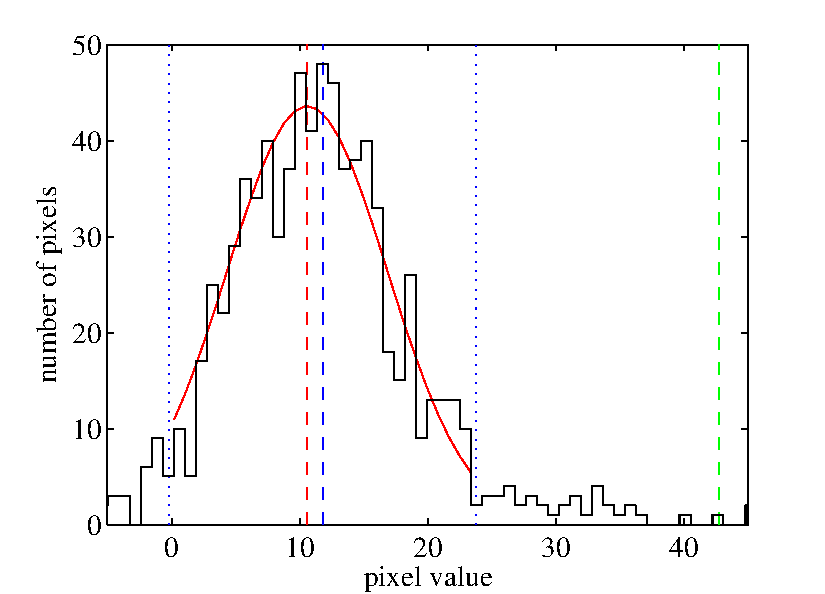
\includegraphics[scale=0.6]{bhist_model.pdf}
\caption{\protect\label{bhist_model} Simulated histogram of pixel
  values in a background block. The model has a true background of
  10mJy with 6mJy Gaussian noise and a single 1Jy source in the
  centre. The red line is the best fit Gaussian.  The fitted peak is
  is 10.3mJy (red dashed line), the median is 11.3mJy (blue dashed
  line), and the mean is 42mJy (green dashed line). The dotted blue
  lines are the $\pm 2 \sigma $ from the median.}
\end{figure}

The fitted peak of the histogram is very insensitive to a small number
of bright sources in the block. As a simple test we made a set of 1000
realizations of a model with a background of 10mJy with Gaussian
random noise with an rms of 6mJy, and put a single 1Jy Gaussian source
in the middle. The resulting histogram for a single realization is
shown in Figure~\ref{bhist_model}. The mean of the block is 42mJy, and
so would give an error of 32 mJy if it were used as the background
estimate. The median is more robust, leading to an error of 1mJy, and
the peak fit is biased by only 0.3 mJy.  It is worth noting that
simple Fourier filter methods, such as the Weiner filter, are
intrinsically linear, and so are approximately equivalent to using the
local mean value as the background estimate. This means that they can be
significantly biased around bright sources.

The background at each pixel is then estimated using a bi-cubic
interpolation between the coarse grid of backgrounds, and subtracted
from the data. 

This approach to background estimateion is similar in principle to the
{\tt nebuliser} algorithm of Irwin (??) 

???

%% Figure \ref{pre_backsub} illustrates the reduction in
%% backgound contamination (mainly arising from galactic cirrus) obtained
%% using this method. 

%\begin{figure}
%\centering 
%\subfloat[Original combined  map]{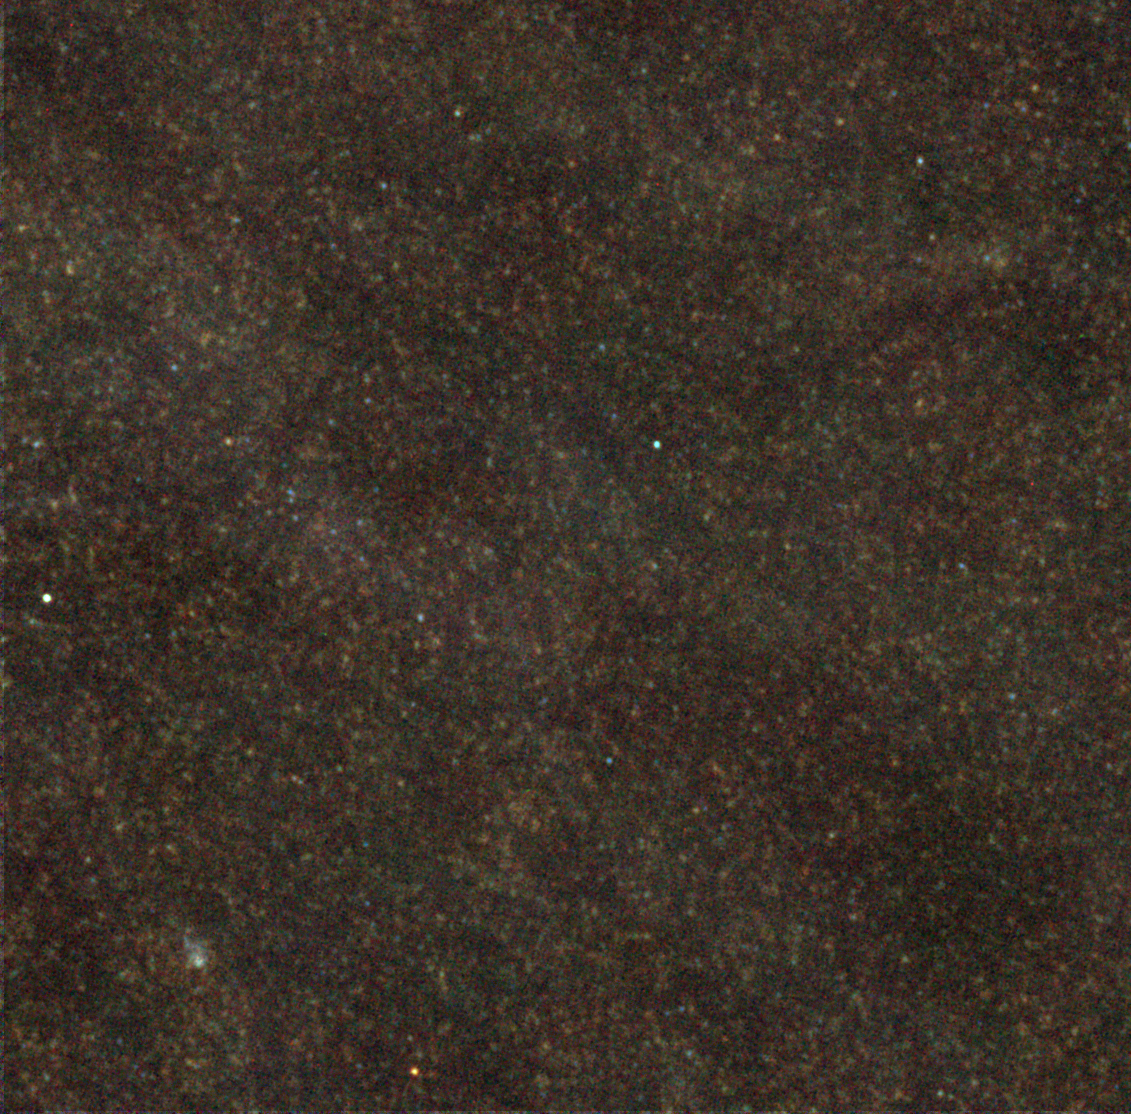
\includegraphics[scale=0.2]{sd_back.png}} \\ 
%\subfloat[After background subtraction]{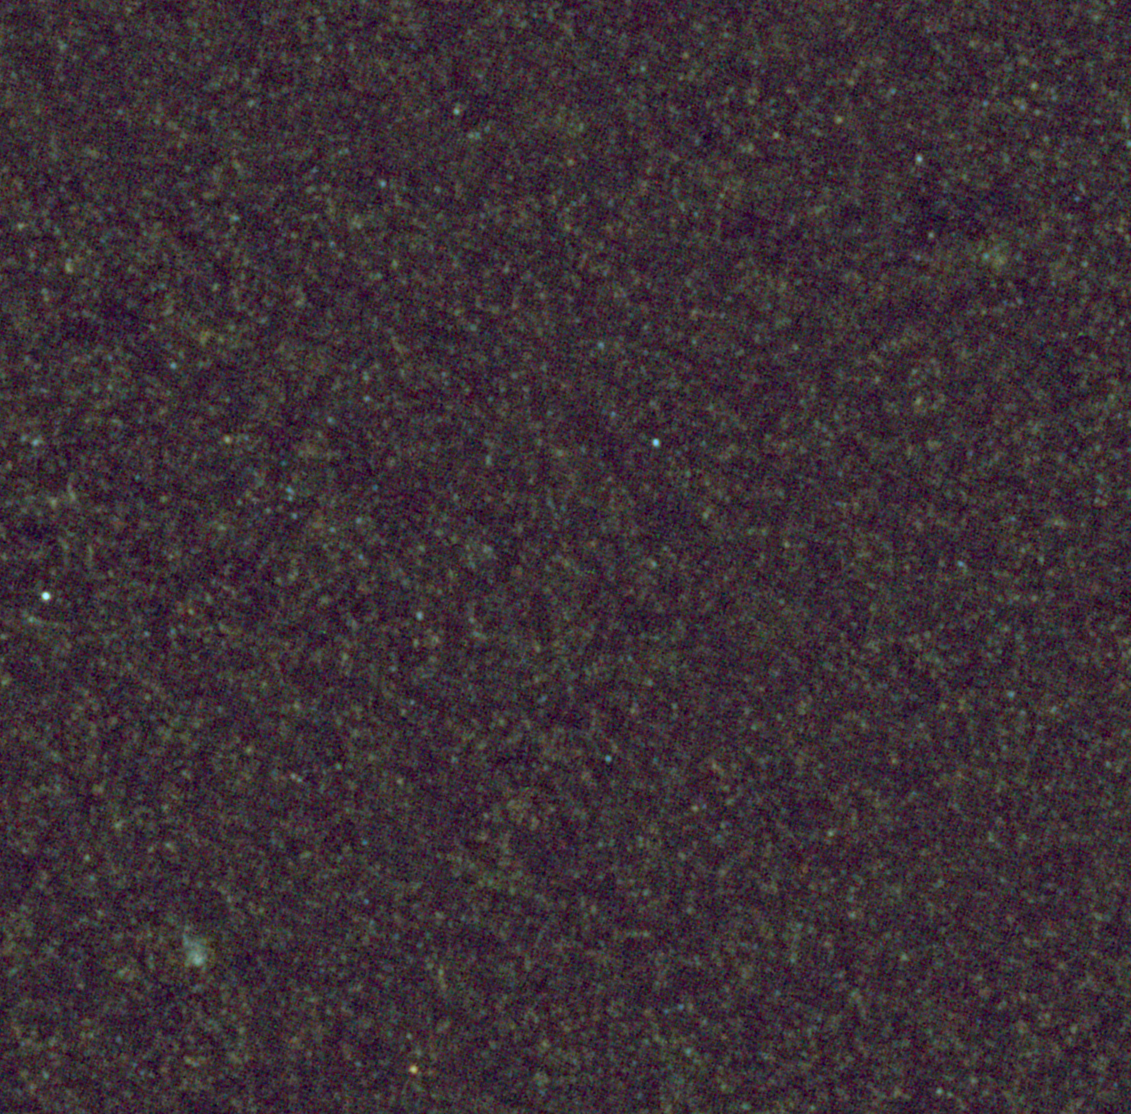
\includegraphics[scale=0.2]{sd_back_new.png}}
%\caption{\protect\label{pre_backsub} False--colour images of a region
%  of the SDP field showing the three SPIRE bands combined (blue: 250 $\mu$m,
%  green: 350 $\mu$m, red: 500 $\mu$m). Image (a) is before
%  background--subtraction and shows clear contamination by galactic
%  cirrus; image (b) shows the effect of subtracting hte
%  background.}
%\end{figure}
%

\section{Filtering}

Typically image data is sampled finely enough that point sources are
sampled by 2 or 3 pixels in each direction. This means that the flux
is spread over several pixels, and the optimal estimate of the source
flux is given by a weighted sum over pixels. Convolving the map by the
right filter function will maximize the signal-to-noise for detecting
sources, and estimating their flux.  For an isolated source on a
uniform background with Gaussian errors, the optimal filter is the
point spread function (PSF), weighted by the inverse of the local
inverse if the variance is spatially varying. In general the optimal
filter may be different from the PSF. For example, when the source
density is high, confusion noise is important, and the optimal filter
is narrower than the PSF. The optimal filter can be estimated using a
Wiener filter approach that includes confusion noise (see Chapmin et
al 2011). The noise-weighted filtered map, $F$, is given by
\begin{equation}
F = \frac{(DW)\otimes P}{W\otimes PQ} ,
\label{filt}
\end{equation}
where $D$ is the background subtracted data in each pixel, the weight
$W=1/\mathrm{var}(D)$ is the inverse of the variance of each pixel,
$P$ is the PSF, and $\otimes$ represents the convolution operator
On the assumption that the instrumental noise on each pixel in the unfiltered
map is uncorrelated, the variance of each pixel in the filtered map is
given by
\begin{equation}
V = \frac{1}{W\otimes PQ} ,
\label{fvar}
\end{equation}
This is a simple generalization  of the PSF-filtering derived by Serjeant
et al (Serjeant et al 2003).


The filtered map gives the minimum $\chi^2$ estimate of the flux that a
source would have at any given pixel in the map. Standard FFT routines
allow easy calculation of the convolved maps at integer pixel
positions, but in practice, sources are not necessarily centered on
pixels. In order to find the best flux estimates, we need to allow for
sub-pixel positioning. Without this, the fluxes will be significantly
underestimated, particularly when a source lies at the edge of a
pixel. Our approach to solving this problem  is discussed in Section 5. 


\section{Combining Wavebands}

The filtered maps provide estimates of source flux and uncertainty at
any position, but they can also be linked to the likelihood ratio of
there being a source at each position rather than background. 
Assuming uncorrelated Gaussian errors, the probability of a part of the
map being simply background is
$$P_b =  \prod \exp \left( -{{1}\over{2}} d_i^2/\sigma_i^2 \right) ,$$
and the corresponding probability of being a point source is  
$$P_s = \prod \exp \left(-{{1}\over{2}} (d_i-s_i)^2/\sigma_i^2
\right), $$ where $s_i$ is the flux distribution of the best-fit point
source, $s_i = F P_i$. The minimum $\chi^2$ value of the source flux
is $F$, given by Eqn\ref{filt}, and the value of $\chi^2$ at the
minimum is $\sum (d_i^2/\sigma_i^2) - F^2/V^2 $.  This means that
maximum $\log$-likelihood ratio of being a source compared to being
background is simply
$$ F^2/2V^2.$$ 
%This can also be considered in terms of the confidence
%limit of there being a source at any position is $F/\sigma$.

This idea can be extended to include any other wavebands that are
available. If we know the observed spectral energy distribution (SED),
$S(\lambda)$ of a source then we can calculate the flux in a band $k$
with response $R_k(\lambda)$,

$$ F_k = \frac{\int S(\lambda) R_k(\lambda) d\lambda } {\int( R_k(\lambda)
  d\lambda } $$ 

Given a set of filters pass-bands, we can calculate the flux in each band. If we
write the normalized SED $S_0(\lambda)= S(\lambda) / \int S(\lambda)
d\lambda$, then the SED of the source is $A S_{0}(\lambda)$, where $A=\int
S(\lambda) d\lambda$. We can also write the broad-band flux in each
band as $AS_{0k}$, where 

$$ S_{0k} = \frac{\int S_{0}(\lambda) R_k(\lambda) d\lambda } {\int( R_k(\lambda)
  d\lambda } $$ 

The values of $S_{0k}$ for each band are the expected fluxes for a
source with the given SED and unit bolometric flux. The expected flux
for any particular source will be $AS_{0k}$. Each individual band
gives an independent estimate of $A$, from the filtered map in that
band. In order to combine the maps, we need to have the independent
estimates at exactly the same position. As discussed in the previous
section, it is best to use a bicubic interpolation to estimate the
source flux at non-integer positions. If we interpolate the lower
resolution maps to the pixels of the highest resolution map, then we
can combine them to obtain the minimum variance estimate of $A$ at any
position in the maps.  For waveband $k$ the estimate of $A$ at
position $x$ is $A_k = F_k(x)/S_{0k}$, and the variance is
$\sigma_{k}^2 = V_k(x)/S_{0k}^2$.  The minimum variance estimate of
$A$ is then given by

$$ A_{tot} = \sum_k{S_{0k}\frac{F_k}{V_k}} \Big/ \sum_k{\frac{S_{0k}^2}{V_k}}$$ 

Note that this includes the factor $S_{0k}$ as part of the weight
given to the waveband $k$ so that the prior expected SED acts as a
weighting term for each band as well as the inverse variance
weighting. This makes intuitive sense: if a source's flux is expected
to peak in a particular band, we should give that band the most weight
in determining the position of the source; if a source has a flat
spectrum, so that the flux is equal in all bands, then all bands are
given equal weight.

The uncertainty on $A_{tot}$ is given by
$$ \sigma_A^2 = \sum_k{\frac{S_{0k}^2}{V_k}},$$ so the significance
of a source detection at any position is $A_{tot}/\sigma_A $. As for a
single band, we can now find the most likely position of the source as
the peak of the combined significance map.  For the whole map, we
first identify all local peaks in the significance map, and retain
those that are $\gtrsim 2\sigma$ as potential sources.  In principle we
could retain all peaks, but rejecting the low-significance peaks gives
a great computational efficiency saving. Next, a variance weighted
least-squares fit of a Gaussian is performed on the $5\times 5$ pixels
around each peak. The position of the peak is allowed to vary freely,
and is not constrained to be at integer pixel positions.  Since the
position can be a non-integer pixel, we fit to the peak to find the
best position at the sub-pixel level.  We fit only to pixels near the
peak to minimize the effects of confusion from other nearby
sources. Since the individual maps have been filtered, the peak pixels
already include data from the surrounding raw pixels in combined in an
optimal way; the peak fitting is solely to find the position at the
sub-pixel level.

In order to estimate the flux in each band, we go back to the filtered
maps, and interpolate to find the value of the map at the position of
the peak in the combined map. If there are sources that are close
together, this simple approach will 'double-count' flux, assigning it
to both source in a pair. A simple way to avoid this is to sort the
sources in order of flux and then subtract off the filtered PSF scaled
by the relevant flux for each source in sequence of decreasing flux.
This is rather like a single-pass 'clean'. In principle, the procedure
could be iterated to a stable solution, but in practice the difficult
cases are blends of sources that require a more sophisticated
de-blending technique to improve the flux estimates. in future
releases we plan to implement multi-source fitting to blended sources.

\section{Sub-pixel subtleties} 



The above anaylsis ignires the complication that our data typically
sample the sky with only 2 or 3 pixels across the FWHM of the psf. In
order to obtain the most accurate estimates of flux and positions, we
need to consider the true flux distribution within each pixel. The
positions are estimated by fitting a Gaussian to central five-by-five
grid of pixels for each detected peak in the map. This provides our
best estimate of the source position, typically to better than 1/10 of
a pixel.

The obvious way to improve on integer positions is to
interpolate between integer pixels. A bilinear interpolation does not
remove the bias, as can be seen by considering a source that is
exactly half way between two pixels; each pixel will have the same
value that less than the true peak value, so the interpolated value
will also be biased low.  A bicubic interpolation allows the
interpolated value to be higher than either individual pixel, and so
gives a better flux estimate. 

The average flux error expected from simply using the value of the
peak pixel can easily calculated, but there will still be a
larger variance introduced by the sub-pixel position of different
sources. Using the bicubic interpolation reduces this scatter and
improves the accuracy of the flux measurements. 

When the psf is sampled into coarse pixels, the value of the peak pixel
is averaged over the whole area of the central pixel, and so is
suppressed relative to the true psf. For a psf tha is close to a
gaussian with 3 pixels across the FWHM, this suppression is typically
$~5\%$. If we use the pixelated psf (the Point Response Function - or
PRF) when filtering the data, this filtered data is boosted by the
suppression factor, and so a source that is centred in a pixel retuns
the correct flux. When a source of not centred in a pixel, the peak
pixel value is supressed more than for a centred source. 

To estimate the flux of the source, we use a bi-cubic interpolation to
find the flux at the source position using the pixels from the filtered
maps. If the source position lies at the boundary between two pixels,
the peak pixel value is suppressed relative to the  peak
of the pixel-centred psf. The bicubic interpolation means that the
estimated flux will be higher than the pixel values, but still a
slight underestimate of the actual peak. As seen in
Figure~\ref{fig:sub-pixel} the error is largest for a source at the
corner of 4 pixels when the flux is underestimated by  $\sim 0.75\%$. 

\begin{figure}
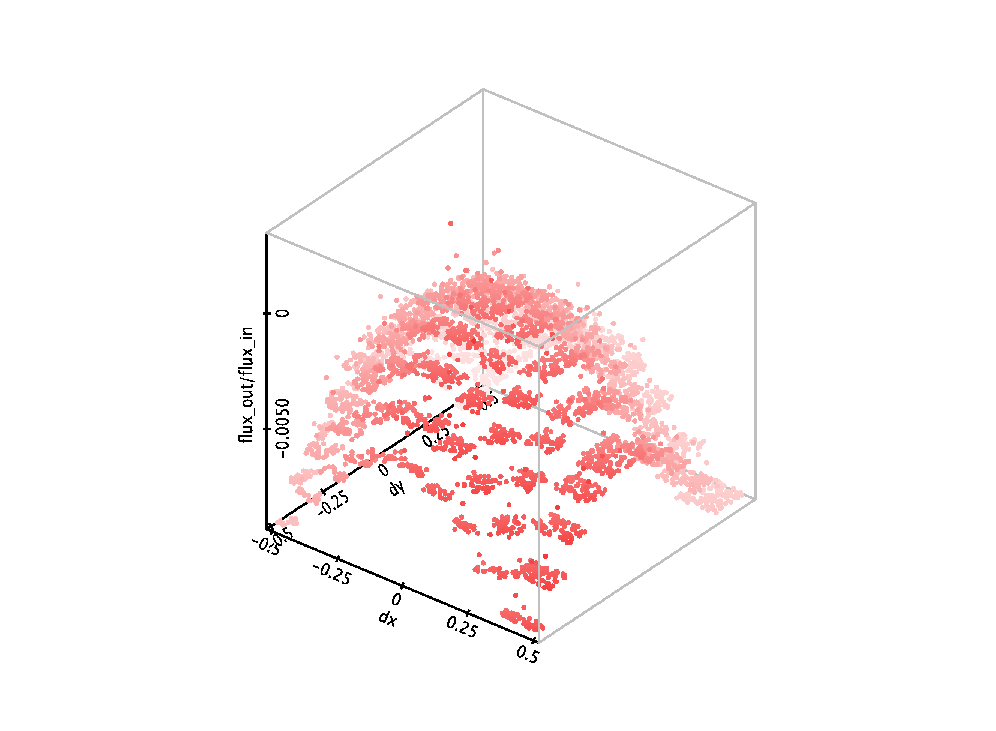
\includegraphics[width=0.5\textwidth]{subpixelposition_fluxerrors1.pdf}
\caption{Fractional flux errors as a function of the precise source
  position within a pixel. The maximum error is $\sim 0.75\%$ for a
  source in the corner of 4 pixels. Sources were placed in the
  simulations at 0.1 pixel positions, which creates the 0.1 pixel
  patches. 
\label{fig:sub-pixel}
}
\end{figure}

\section{Tests of the method} 

As a simple test of the source detection we generated maps in 3
far--infrared and submillimetre bands (250, 350 and 500
$\mu$m) each map containing isolated sources on a grid of positions.

The sources are assigned random positions near the grid centres, so
that the pixels sample the psf with random offsets from the pixel
centres.  Each source is given a 250\mic flux between 1mJy and 1Jy,
uniformly spaced in log flux. The 350\mic and 500\mic fluxes for each
source are then assigned so that the SED matches a modified black body
with $\beta$ chosen from a uniform random distribution between 1 and
2, and temperature, $T$, randomly chosen from a lognormal distribution
centred on $T=25$K, and ranging from 15K to 40K, as shown in
Fig~\ref{fig:Tdist}. This distribution roughly matches the SEDs of
low-redshift galaxies seen in the Herschel-ATLAS survey (Smith et al 2012). 
To represent higher redshift galaxies, which appear much redder, we
set $f_{350}= 2f_{250}$ and $f_{500} = 3 f_{500}$. This matches the
typical FIR colours for a z=4 galaxy. 


\begin{figure} 

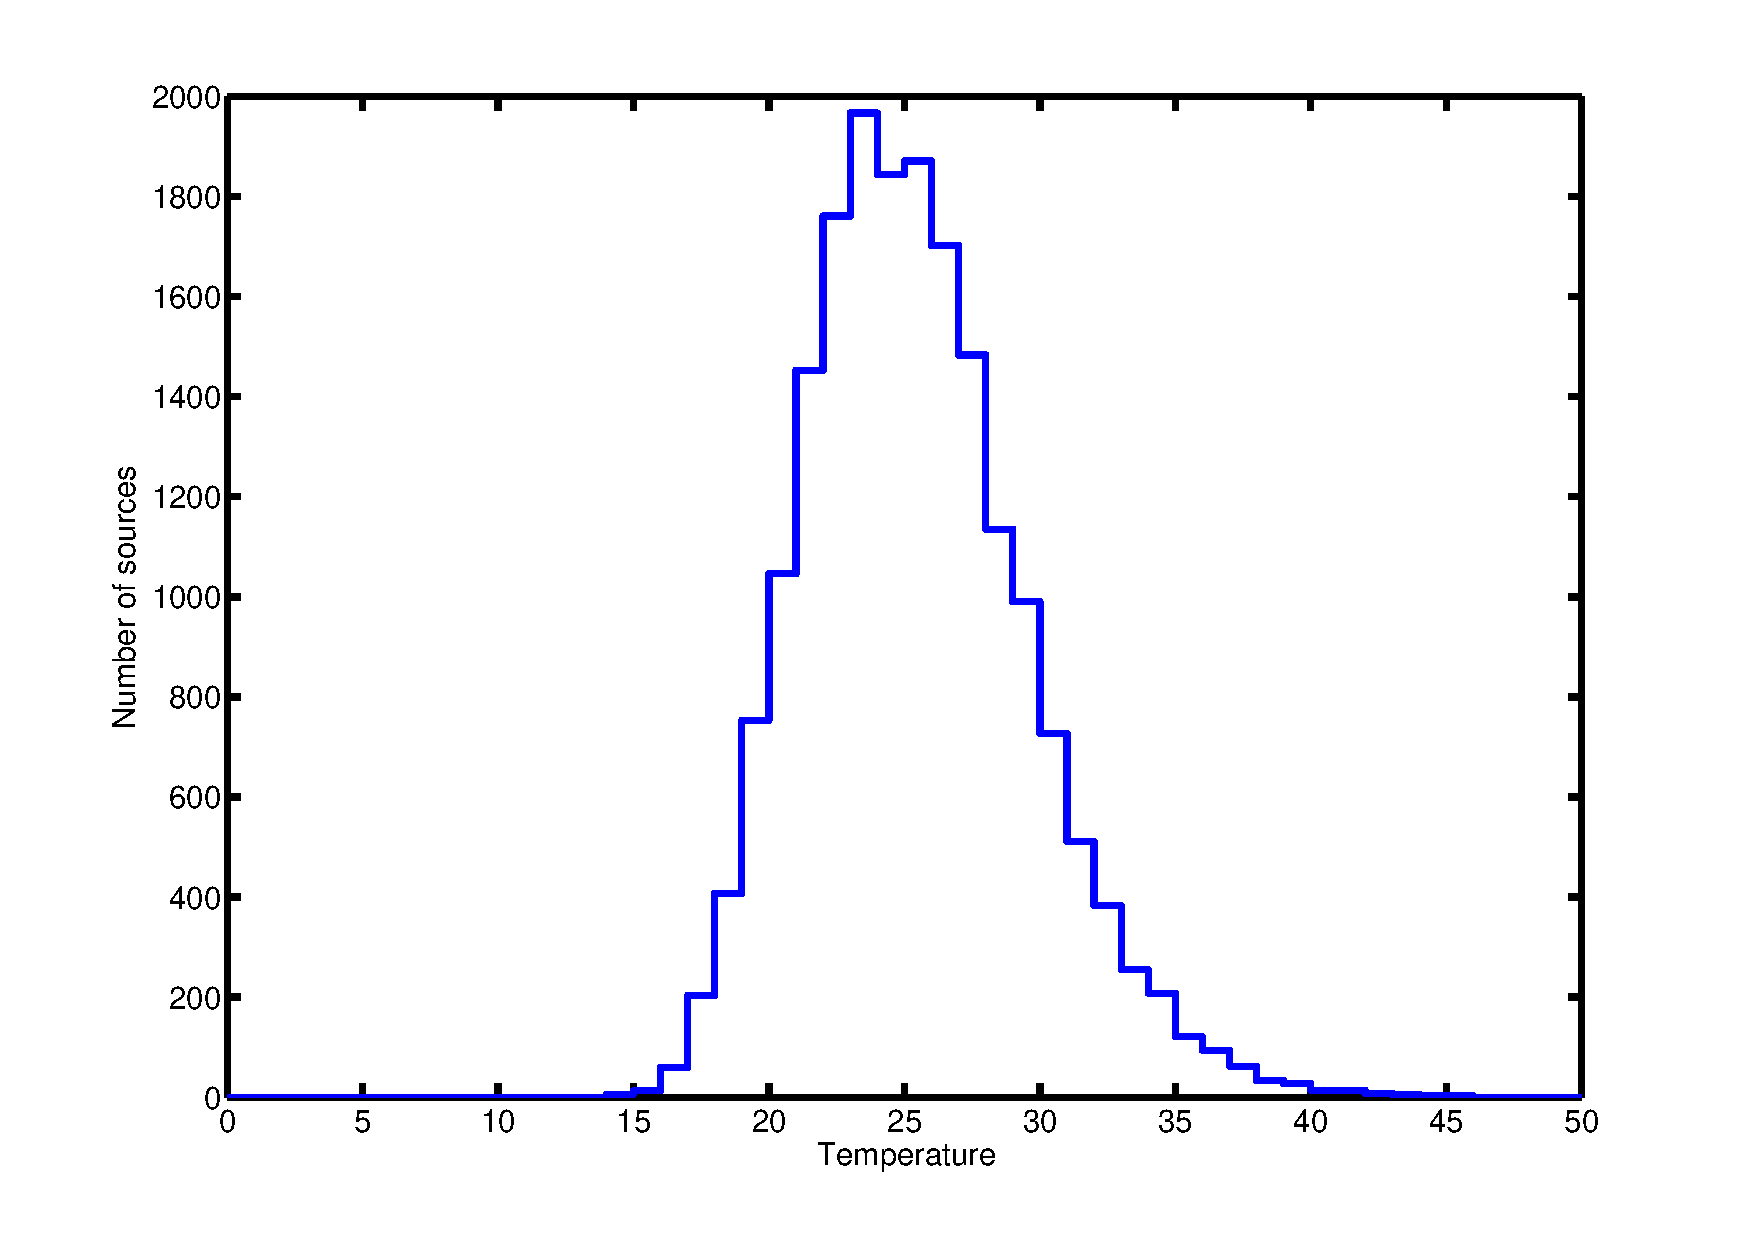
\includegraphics[width=0.4\textwidth]{Temp_dist.pdf} 
\caption{The temperature distribution of simulated sources. 
\label{fig:Tdist}}
\end{figure}

We also added a galactic background by taking the SFD 100~$\mu$m and
temperature maps and scaling the 100~$\mu$m emission to the relevant
wavelength using a modified black-body. The resolution of the SFD maps
is several arcminutes, and so does not contain small-scale structure
in the cirrus background. The HATLAS data show that in some patches of
sky there is strong cirrus emission with significant structure on
sub-arcminute scales, but in most areas, the emission is relatively
smooth. Our simulated background is a reasonable approximation for
most of the sky, but will be somewhat easier to subtract than the
areas where the true cirrus is particularly strong and structured.

Finally we add Gaussian noise to the maps. The standard deviation is
varied by $\sqrt{N_\mathrm{passes}}$, where $N_\mathrm{passes}$ is
the number of passes contributing to a pixel in a typical coverage map
for the HATLAS survey data.

We then run MADX on the simulated maps to detect the input sources and
measure their position and fluxes. A simple positional match allows us
to associate the detected sources to the to the corresponding input
sources, and so calculate the errors in position and fluxes. Since we
put the sources on a randomized grid, there is no possibility of
confusing one source with another. We used two different priors: first
just using only the 250\mic band for the detection (weights 1,0,0);
and second, equally weighting each band (weights 1,1,1). For each run,
we measure the completeness by simply counting the fraction of input
sources that are detected as a function of
flux. Figure~\ref{fig:completeness} shows the completeness as a
function of the signal to noise in the 250\mic band.

\begin{figure} 
(a) 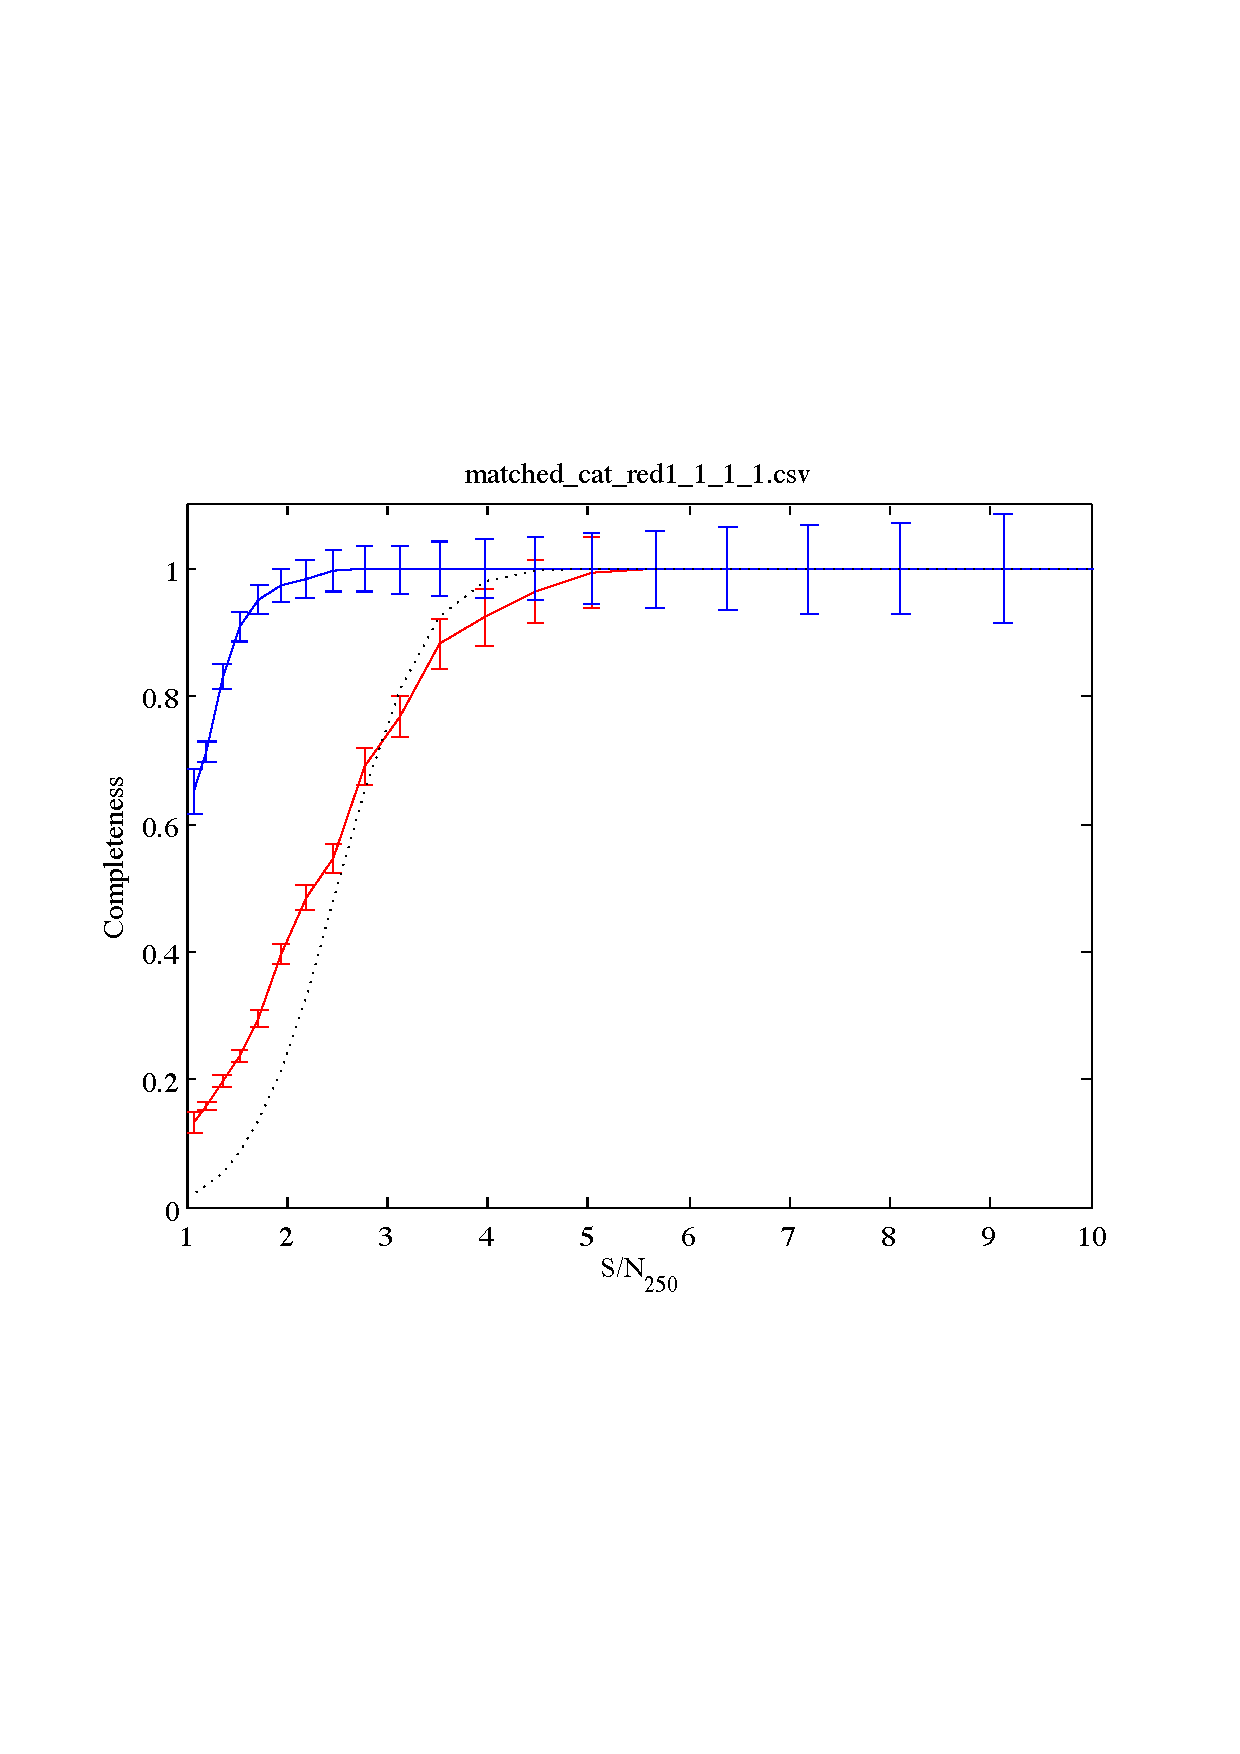
\includegraphics[valign=t,width=0.4\textwidth]{completeness1_100_111.pdf}\\
(b) 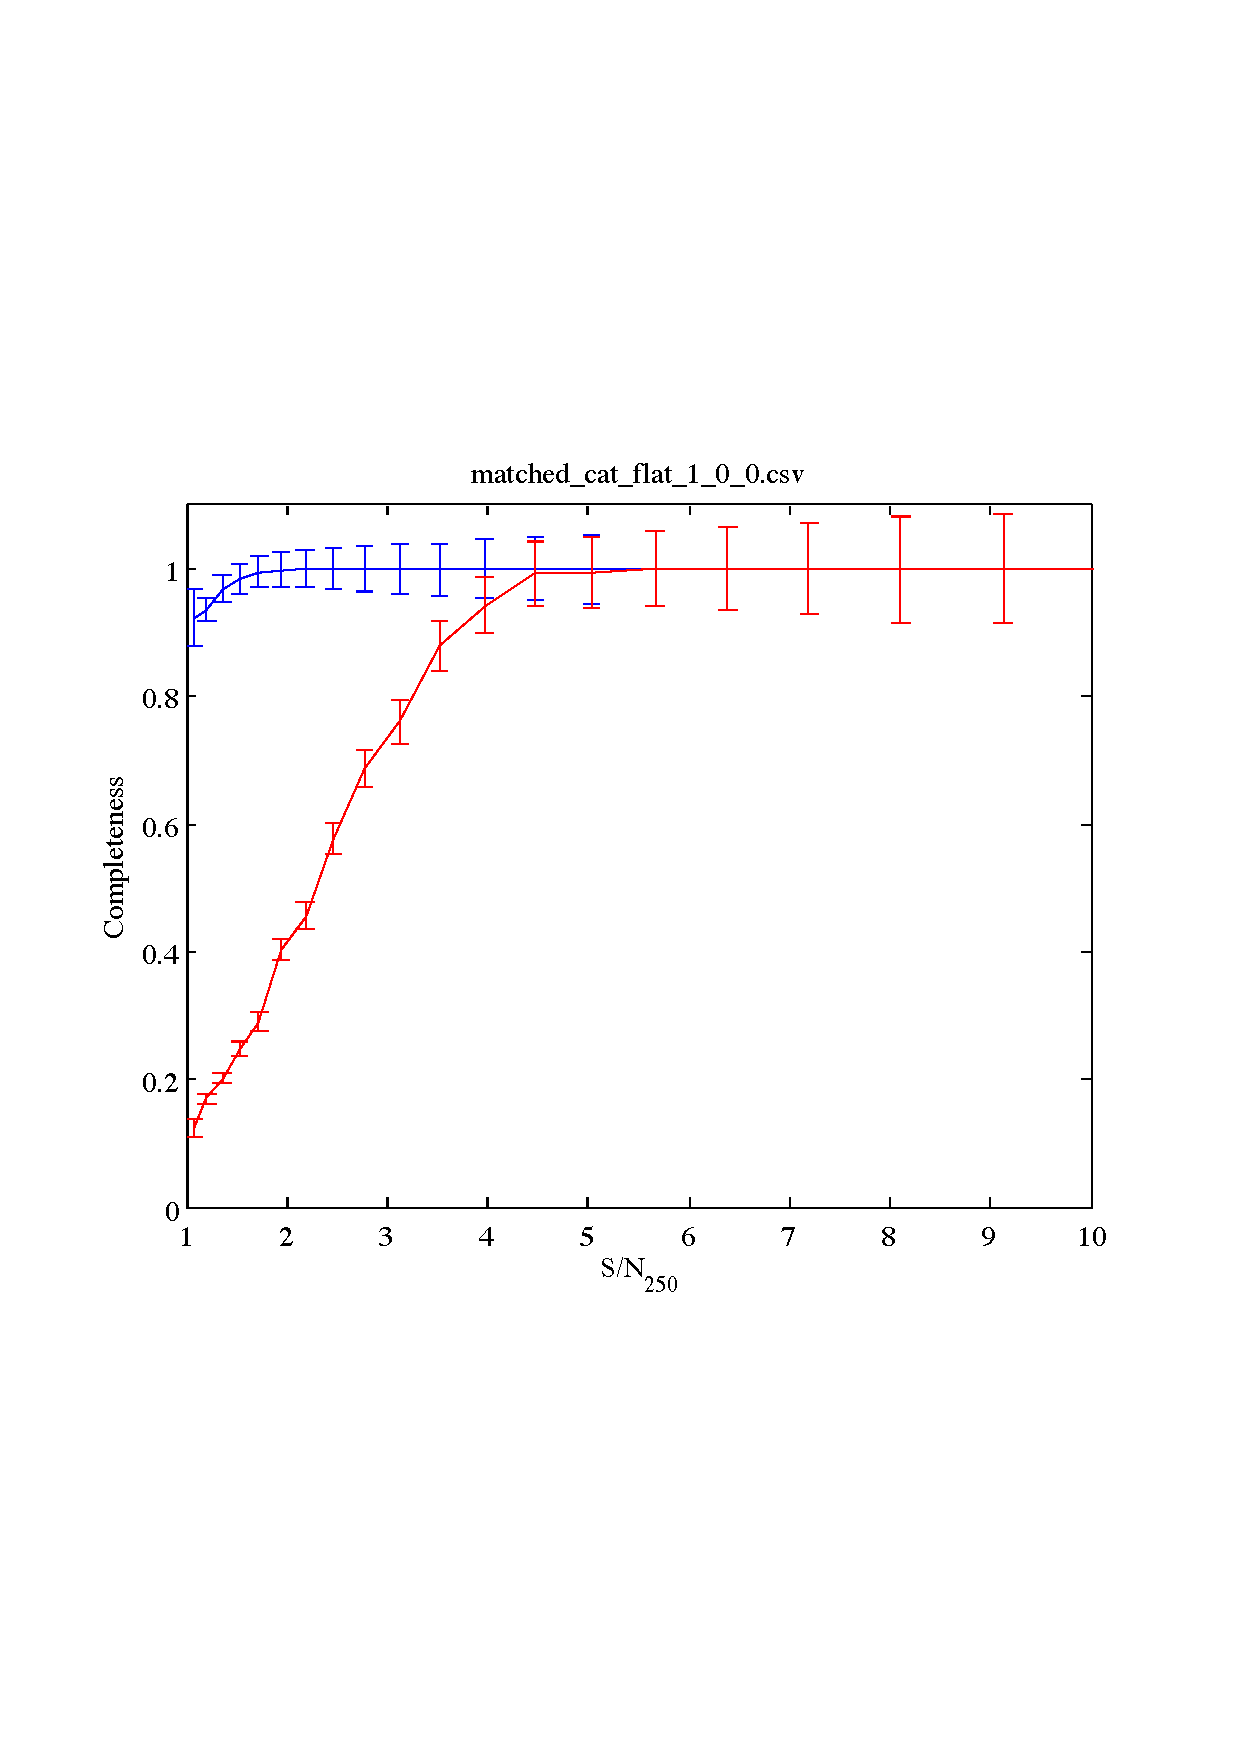
\includegraphics[valign=t,width=0.4\textwidth]{completeness_red_sources.pdf}
\caption{}
\label{fig:completeness}
\end{figure}

It is clear that including information from all three bands
significantly improves the completeness of the resulting
catalogue. For sources with a red SED the gain is a factor 3 in
signal-to-noise in the 250\mic band. 

Next we compare the measured positions to the input positions. It may
be thought that including data from lower resolution bands would
increase the positional errors, but by using the correct weighting
between the bands, the extra information actually improves the
positional accuracy. This can be seen in Fig~\ref{fig:positions},
which shows the rms position error in ra and dec as a function of
signal-to-noise.  
\begin{figure} 
(a)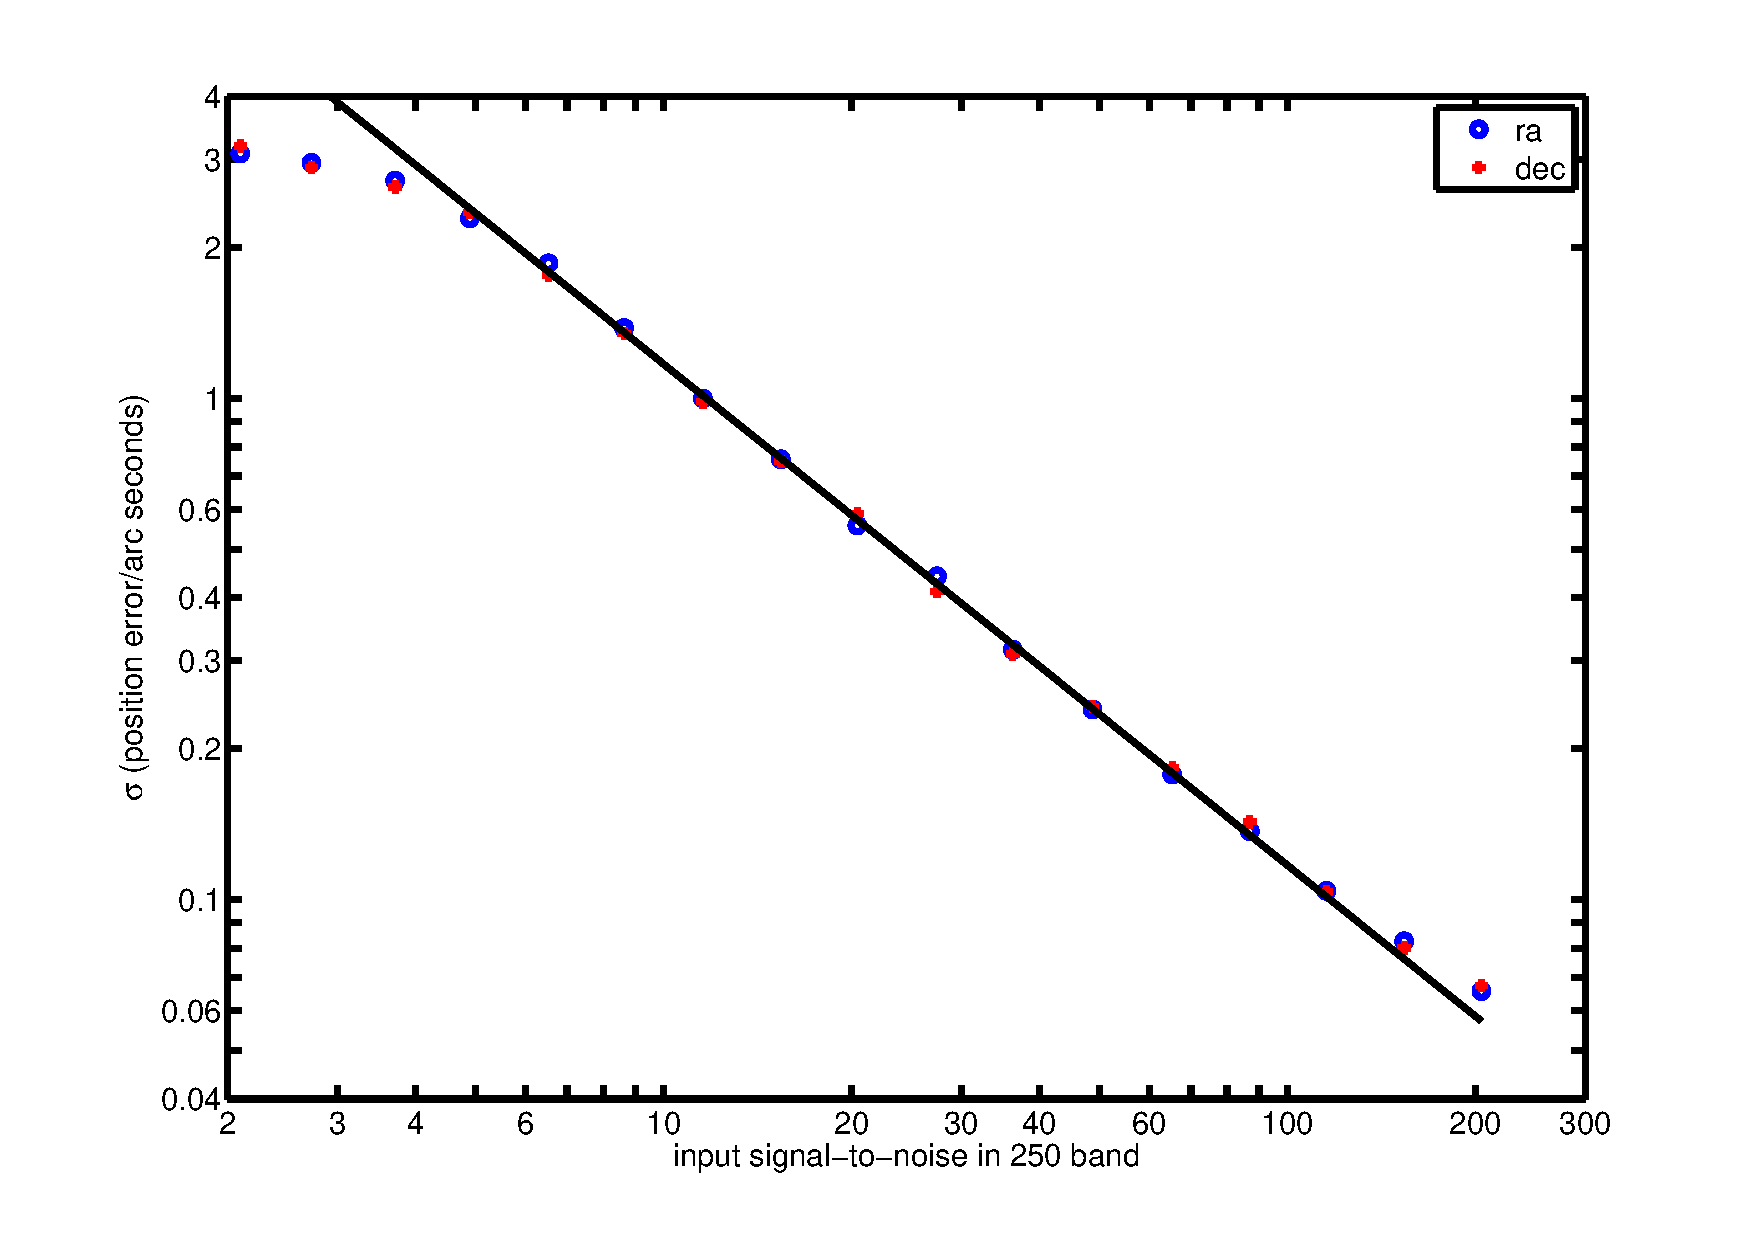
\includegraphics[width=0.4\textwidth]{posn_errors_100.pdf}\\
(b)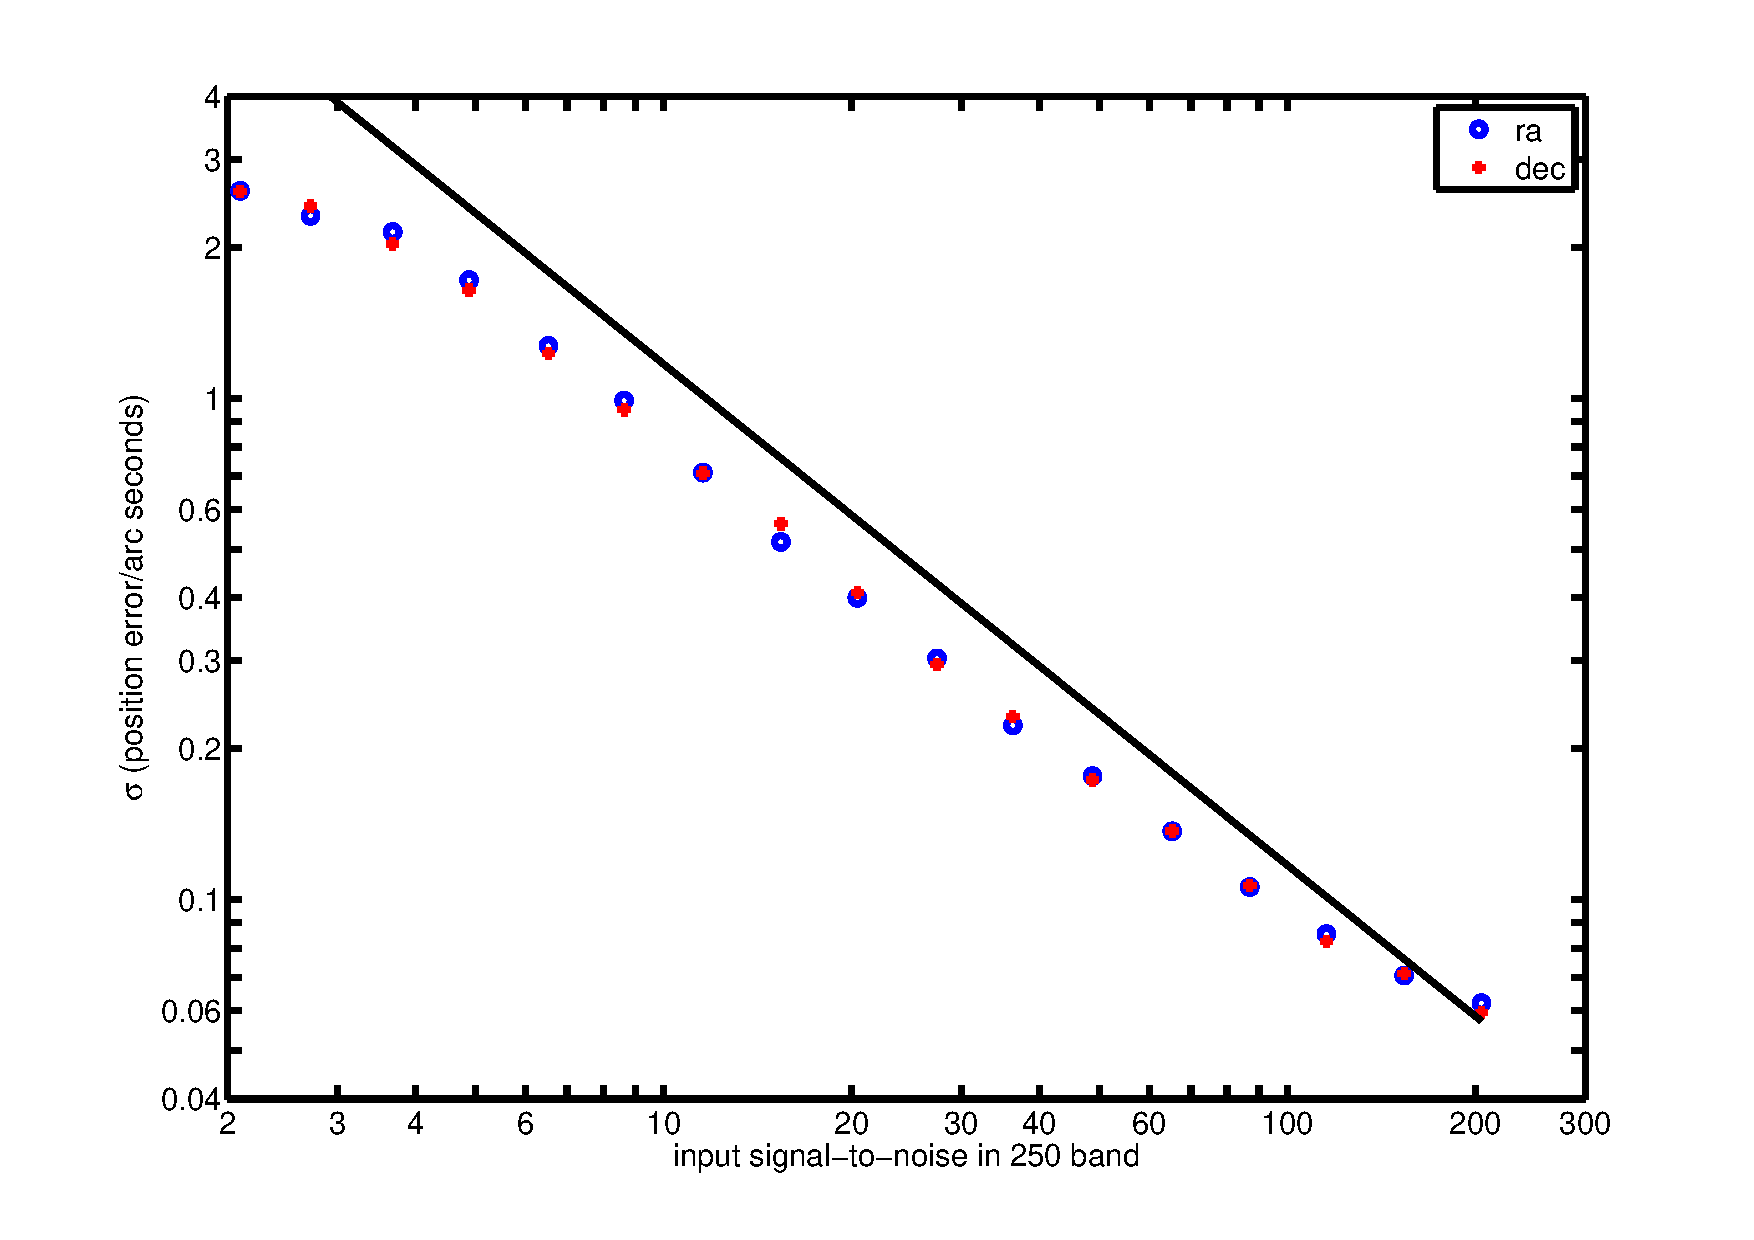
\includegraphics[width=0.4\textwidth]{posn_errors_111.pdf}
\caption{
\label{fig:positions}
The measured positional errors of simulated sources plotted as a
function of signal-to-noise in the 250\mic band. The standard
deviation of the errors in ra are shown as blue circles, and in dec
shown as red crosses.  Panel (a) shows the measurements using only the
250 band to detect sources and measure their positions. Panel (b)
shows the measurements using the flat-prior detection. The black line
in both panels shows the variation expected from the theoretical
analysis of  Ivison (2007). }
\end{figure}

\begin{figure} 
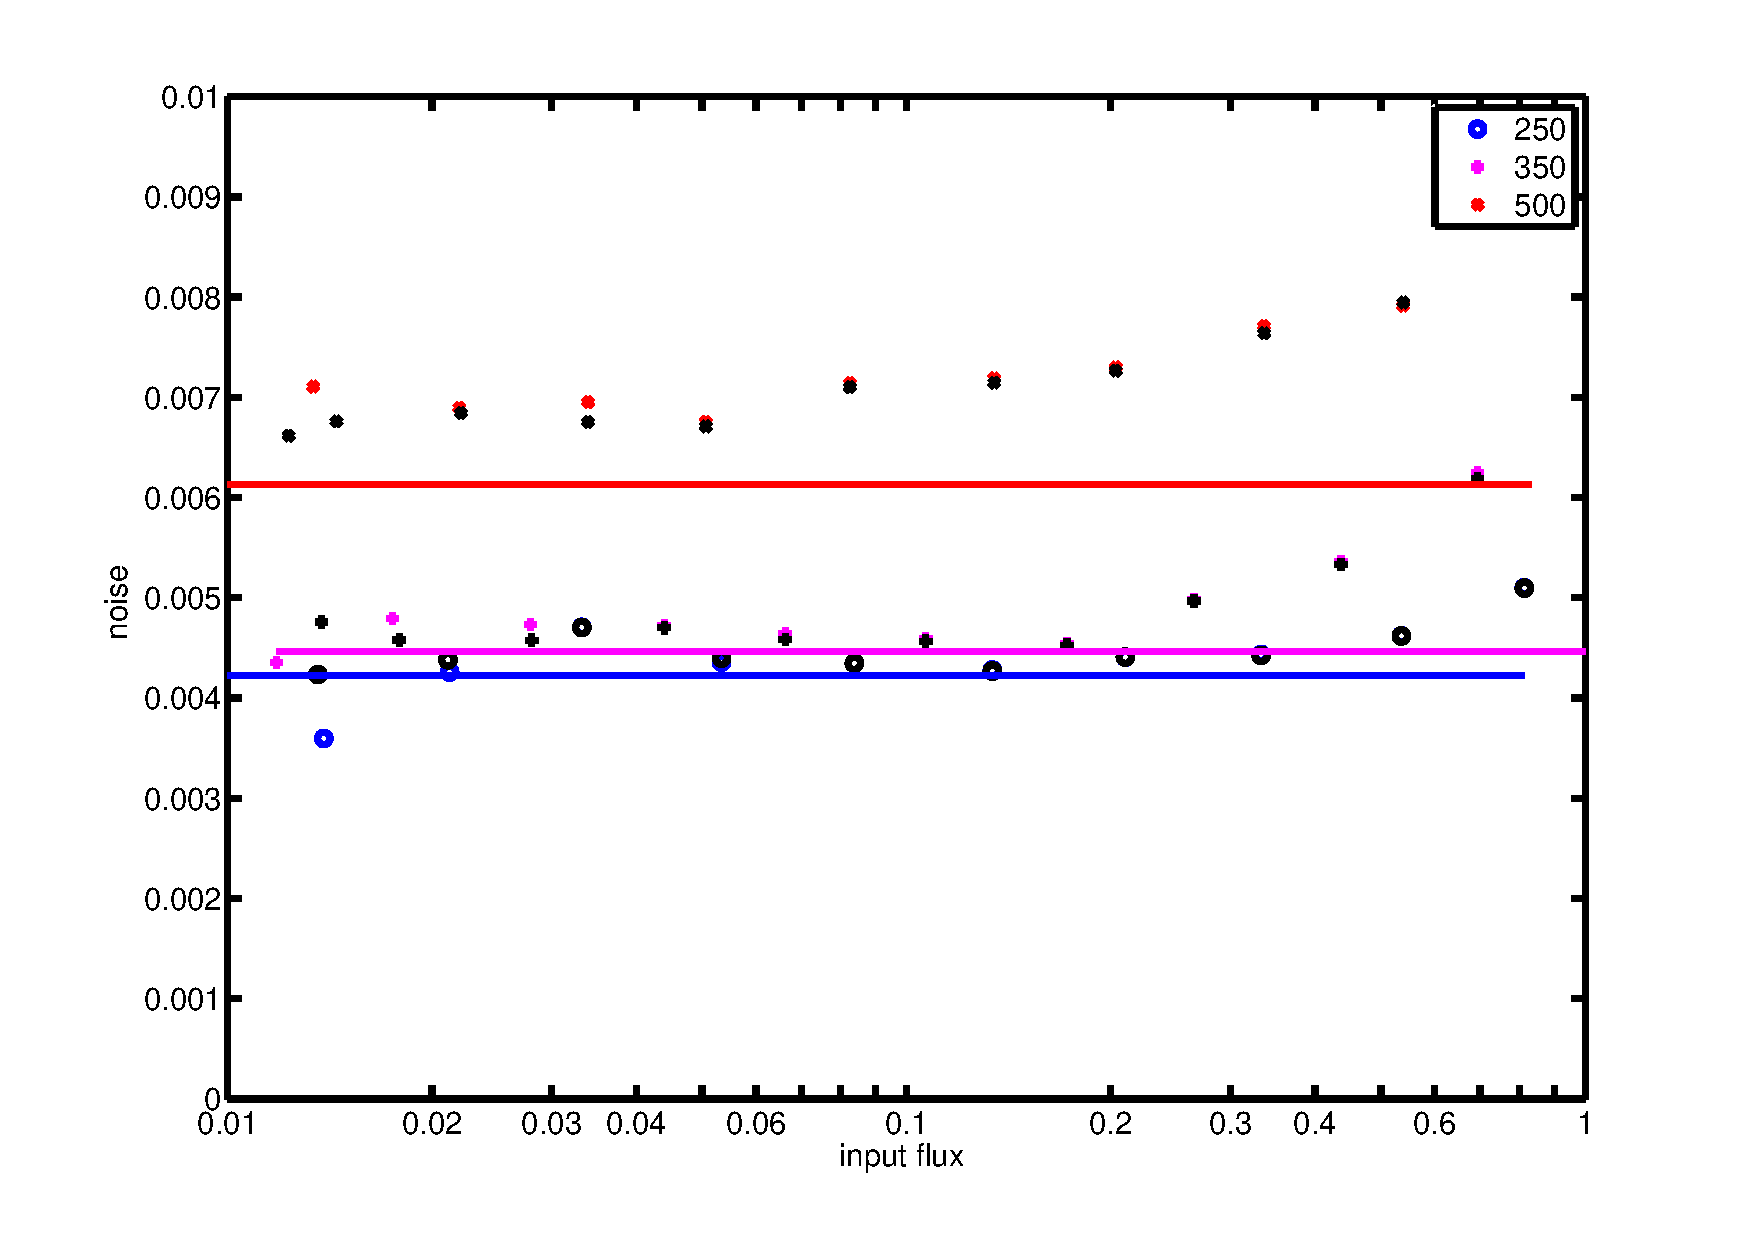
\includegraphics[width=0.4\textwidth]{noise_comparison.pdf}
\caption{
\label{fig:sn}
The measured signal to noise for each band measured as a function of
input signal-to-noise in the 250 band. The expected The flat-prior and 250 only
detection choice makes little difference in the resulting flux errors.

}
\end{figure}


Finally we compare the measured and input fluxes for the sources, in
terms of both random and systematic errors. We compute the rms
deviation of between the measured and input 250\mic flux as a function
of the expected noise given the input Gaussian errors per pixel.  As
shown in Fig~\ref{fig:sn}, the random errors match the input gaussian
error for fainter sources. For brighter sources the fractional errors
from the sub-pixel positioning begin to dominate, and the measured
errors are larger than the Gaussian errors.  The choice of prior makes
little difference in the errors on the flux measurements, as the
errors are dominated by the pixel errors on the map for each band. The
exception is for faint 250\mic fluxes and the 250\mic only prior. The
measured standard deviation for these sources is biased low because
many sources with negative noise values fall below the detection
threshold, and so do not contribute to the measured standard
deviation, leading to an artificially low estimated noise.  Using the
flat prior mitigates this problem and the measured noise continues to
match the expected noise to the lowest fluxes.  The random noise on
the 350\mic fluxes also match the expected noise. For the 500\mic
band, the measured errors are 10\%  higher than expected

Fig~\ref{fig:fluxes} shows the mean ratio of measured to input flux as
a function of signal to noise. At high signal to noise there is a
small underestimate of flux due the peak pixelization issues discussed
in section 5.  For fainter sources near the detection limit, there is
a systematic bias to higher fluxes (flux boosting). This is related to
Eddington/Malmquist bias from when selecting only sources above a
signal-to-noise threshold: faint sources with negative errors are not
retained in the catalogue, whereas those with positive errors are
detected to a fainter level.  The precise form of the boosting depends
on the distribution of true source fluxes, as well as the measurement
errors.  For the simulations used here we chose to distribute sources
uniformly in log flux, and so they do not match real source flux
distributions, even though the colours are realistic. Hence we cannot
use them to estimate the boosting as a function of flux for real
data. Valiente et al (2016) a created realistic simulations and used
them to estimate both completeness and boosting correction factors
that apply to real data.

For the other two bands, there is a similar small bias at high signal
to noise, caused by peak pixelization effects. For fainter sources,
there is a larger negative bias which is caused by positional errors,
which mean that the local peak is missed and the flux estimate is
systematically too low.


\begin{figure}
(a)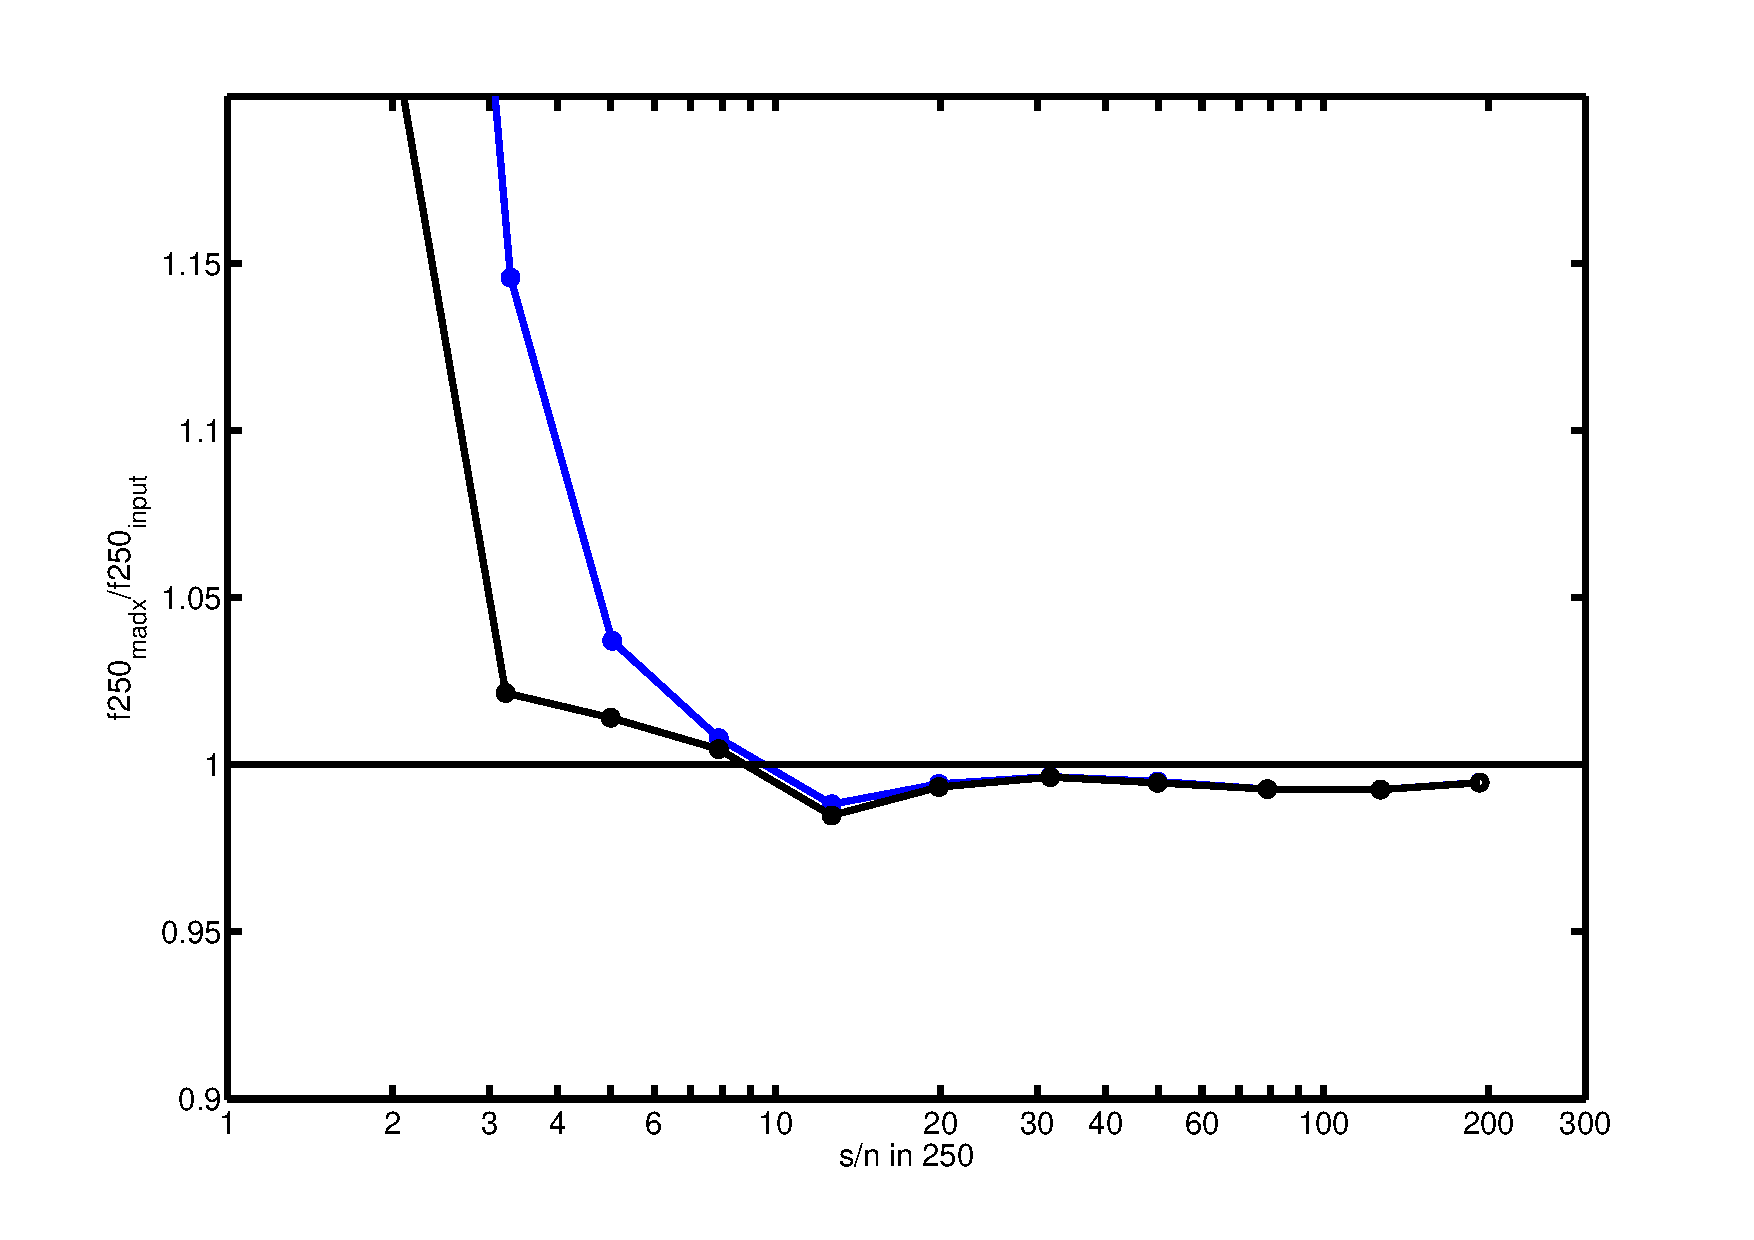
\includegraphics[width=0.4\textwidth,valign=t]{flux_bias250.pdf}
(b)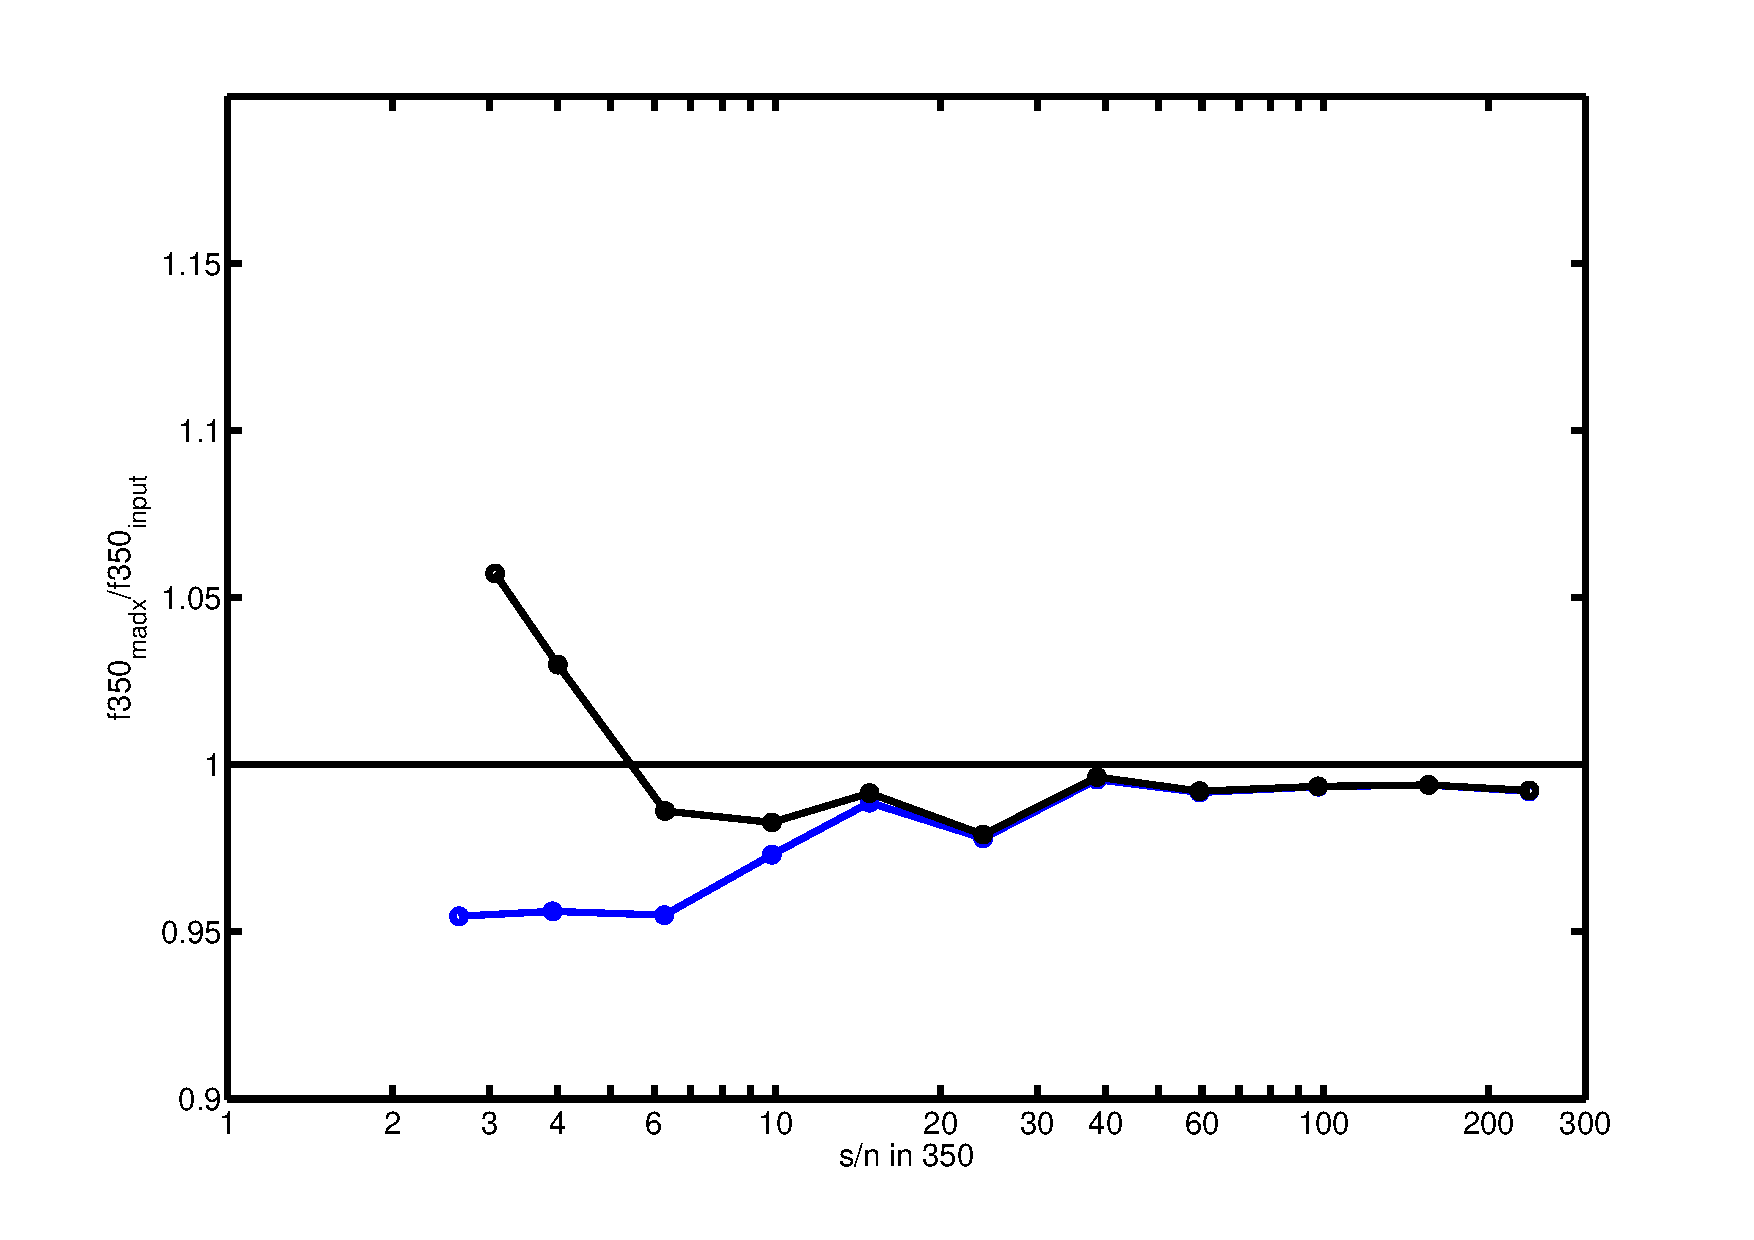
\includegraphics[width=0.4\textwidth,valign=t]{flux_bias350.pdf}
(c)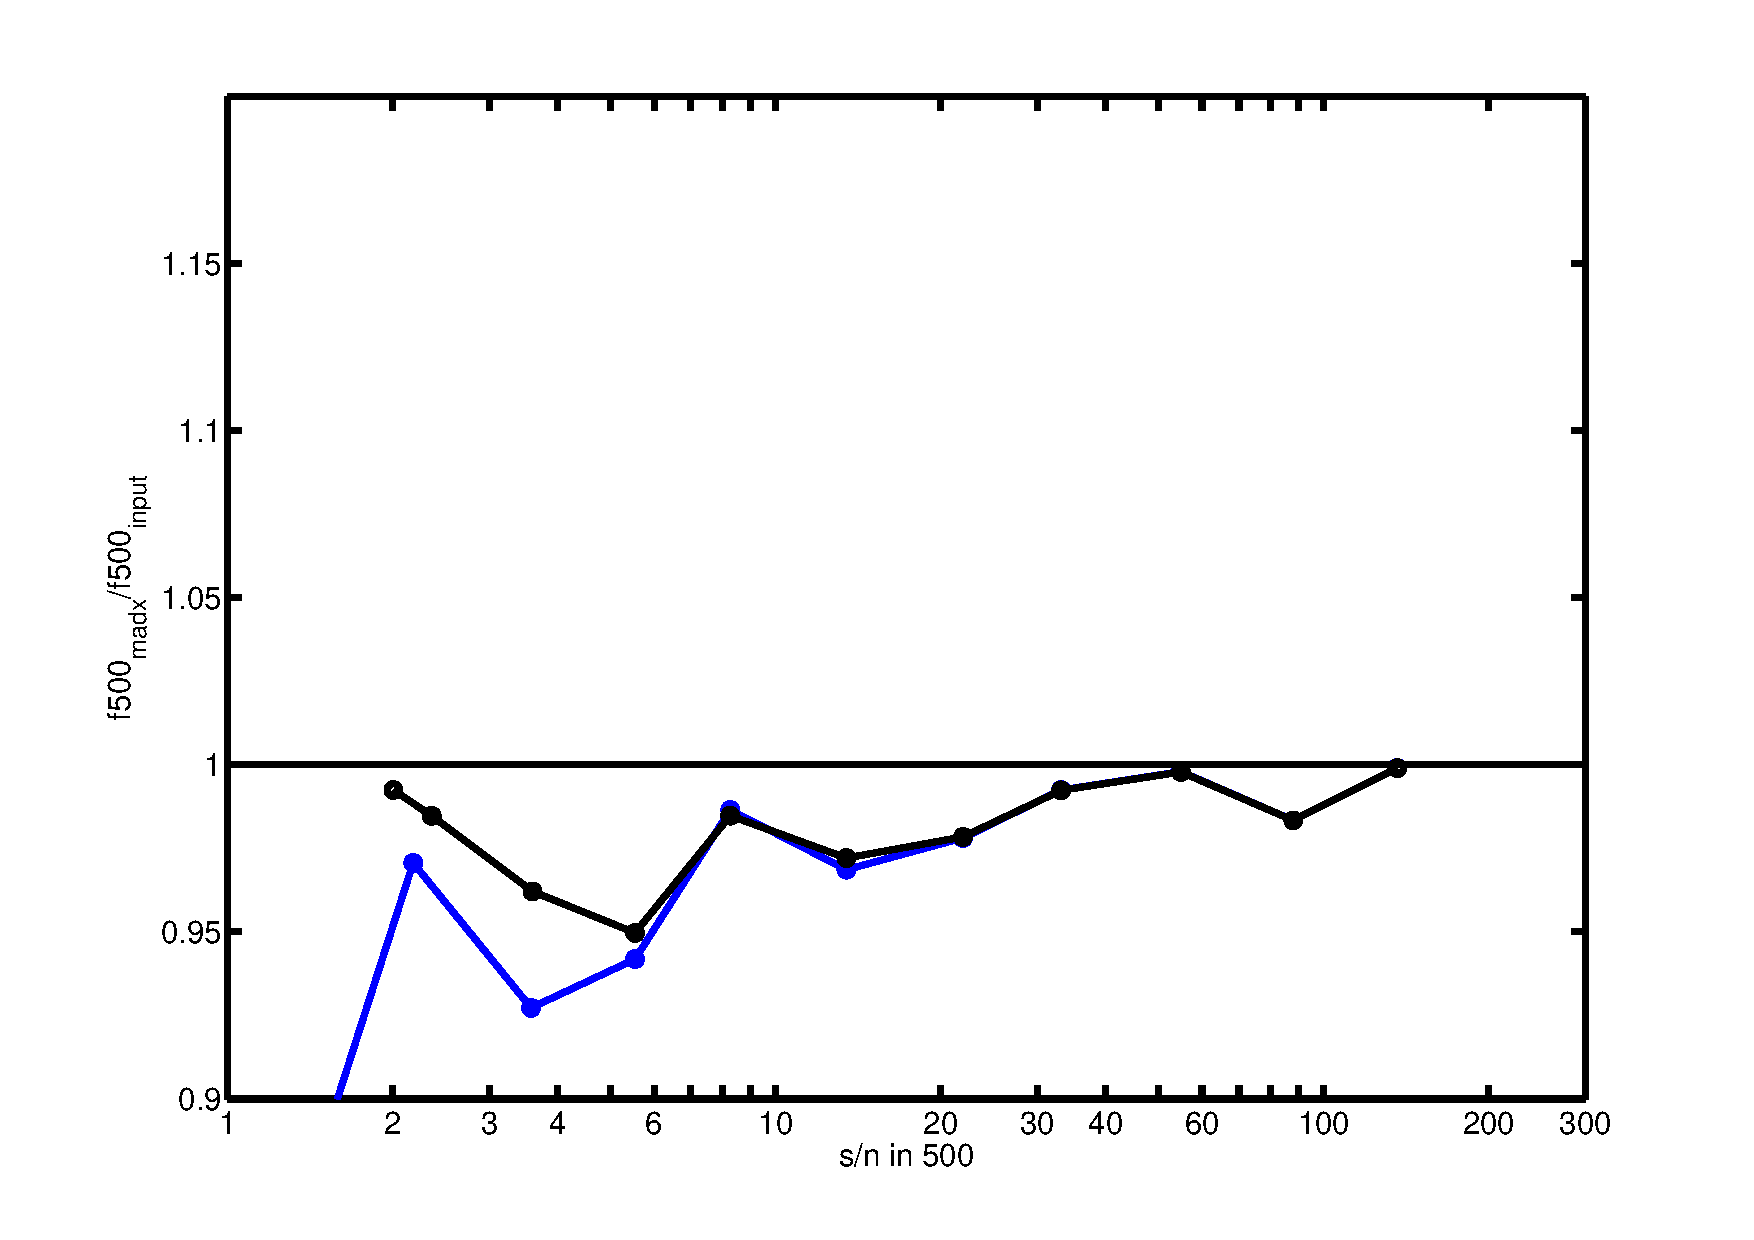
\includegraphics[width=0.4\textwidth,valign=t]{flux_bias500.pdf}
\caption{\label{fig:fluxes} 
The ratio of mean measured flux compared to the mean input flux as a
function of input signal to noise for two source detection priors. The
blue line uses only the 250 band, and the black line uses a flat
prior. Panel (a),(b) and (c) shows the results for the 250\mic, 350\mic
and 500\mic fluxes respectively. Using the
flat prior reduces the boosting effect at fainter fluxes. 
}

\end{figure}

%\section*{Acknowledgments}


\begin{thebibliography}{}

\bibitem[Bertin \& Arnouts(1996)]{sext} Bertin, E., \& Arnouts, S.\ 1996, \aaps, 117, 393 

\bibitem[Clements et al.(2010)]{clements} Clements, D.~L., et  al.\ 2010,  A\&A, in press, arXiv:1005.2409 

\bibitem[Driver et al. (2009)]{gama}Driver, S.P., et al., 2009,
  Astron. Geophys.,  50, 5.12

\bibitem[Dunne et al (2000)]{slugs} Dunne, L., Eales, S. A., Edmunds,
  M., Ivison, R., Alexander, P., \& Clements, D. L. 2000, MNRAS, 315,
  115

\bibitem[Dye et al. (2009)]{dye}Dye, S., et al., 2009 ApJ., 703, 285

\bibitem[Eales et al.(2010)]{eales} Eales, S., et al.\ 2010,  \pasp, 122, 499 

\bibitem[Griffin et al. (2010)]{spire} Griffin et al. 2010 A\&A this issue.

\bibitem[Ibar et al. (2010)]{pacsmaps} Ibar, E., 2010, MNRAS, submitted

\bibitem[Ivison et al.(2007)]{ivison} Ivison, R.~J., et al.\ 2007, \mnras, 380, 199 

\bibitem[Maddox et al.(2010)]{wtheta} Maddox, S.~J., et al.\  2010,  A\&A, in press, arXiv:1005.2406 

\bibitem[Negrello et al.(2007)]{negrello} Negrello, M., 
Perrotta, F., Gonz{\'a}lez-Nuevo, J., Silva, L., de Zotti, G., Granato, 
G.~L., Baccigalupi, C., \& Danese, L.\ 2007, \mnras, 377, 1557 

\bibitem[Ott et al. (2010)]{hipe} Ott, S. 2010, in ASP Conference Series, Astronomical Data Analysis 
Software and Systems XIX, Y. Mizumoto, K.-I. Morita, and M. Ohishi, eds., in press 

\bibitem[Pascale et al. (2010)]{spiremaps}Pascale, E., et al, 2010, MNRAS, submitted

\bibitem[\protect\citeauthoryear{{Pilbratt}}{{Pilbratt et al.}}{2010}]{herschel} Pilbratt, G.~L., et al. A\&A in press, arXiv:1005.5331 

\bibitem[Poglitsch et al. (2010)]{pacs} Poglitsch, A., et al. 2010 A\&A, in press, arXiv:1005.1487 

\bibitem[Rigby et al. (in prep)]{rigby} Rigby, E.E, et al., MNRAS. 

\bibitem[Rowan-Robinson (2001)]{rr} Rowan-Robinson, M. 2001, in IAU
  Symp. 204, The Extragalactic Infrared Background and its
  Cosmological Implications, ed. M. Harwit \& M. G.  Hauser (Dordrecht:
  Kluwer), 265


\bibitem[Schlegel et al.(1998)]{iras_ref} Schlegel, D.~J., 
Finkbeiner, D.~P., \& Davis, M.\ 1998, \apj, 500, 525 

\bibitem[Smith et al. (2010)]{Smith} Smith, D et al, 2010,  MNRAS, in prep

\bibitem[Wang \& Rowan-Robinson(2009)]{iras} Wang, L., \& Rowan-Robinson, M.\ 2009, \mnras, 398, 109 

\end{thebibliography}
\label{lastpage}

\end{document}

